
%%%%%%%%%%%%%%%%%%%%%%%%%%%%%%%%%%%%%%%%
\documentclass{paper}
%%%%%%%%%%%%%%%%%%%%%%%%%%%%%%%%%%%%%%%%

% Declare some TeX packages needed for graphics. 
\usepackage[pdftex]{graphicx}
\usepackage{epstopdf}
\usepackage{grffile}
\epstopdfsetup{suffix=}

%\ifx\pdftexversion\undefined
%   \usepackage[dvips]{graphicx}
%\else
%   \usepackage[pdftex]{graphicx}
%   \usepackage{epstopdf}
%   \epstopdfsetup{suffix=}
%\fi

%%%%%%%%%%%%%%%%%%%%%%%%%%%%%%%%%%%%%%%%
\begin{document}
%%%%%%%%%%%%%%%%%%%%%%%%%%%%%%%%%%%%%%%%


\section{Project Overview}
This is the output of the Project Analysis R file used to run the analysis of my project.


My analysis begins with some summary statistics on the dataset I chose for my project:


\begin{figure}
\centering
\includegraphics[width=\textwidth]{../Figures/HistogramCallsforAllNames.eps}
\caption{Calls for All Names}
\label{fig:allcalls}
\end{figure}


\begin{figure}
\centering
\includegraphics[width=\textwidth]{../Figures/Histogram-CallsforCaucasianNames.eps}
\caption{Calls for Caucasian Names}
\label{fig:whitecalls}
\end{figure}


\begin{figure}
\centering
\includegraphics[width=\textwidth]{../Figures/Histogram-CallsforAfricanAmericanNames.eps}
\caption{Calls for African American Names}
\label{fig:blackcalls}
\end{figure}


This gives a little insight into the data, but I will further explain here. This dataset is the result of sending 4870 randomized resumes to employers in the Chicago and Boston area for numerous jobs. What is being analyzed here? Whether or not these resumes garnered a call back based on the first name listed on the resume. Half of the resumes have what Americans would consider a white or Caucasian name, while the other half have an African American name associated with it. I am using the 'call' variable - a binary 'yes' or 'no' data value - as the dependent variable for my analysis.


\section{Analysis}


Here are some summary statistics on the explanatory variables within this dataset that I have hand-picked from the full dataset for this project:


% latex table generated in R 3.6.1 by xtable 1.8-4 package
% Sat Dec 05 18:24:24 2020
\begin{table}[ht]
\centering
\begin{tabular}{rllllll}
  \hline
 &      name &    gender & ethnicity & quality &      city &      jobs \\ 
  \hline
X & Tamika : 256   & female:3746   & afam:2435   & high:2446   & boston :2166   & Min.   :1.000   \\ 
  X.1 & Anne   : 242   & male  :1124   & cauc:2435   & low :2424   & chicago:2704   & 1st Qu.:3.000   \\ 
  X.2 & Allison: 232   &  &  &  &  & Median :4.000   \\ 
  X.3 & Latonya: 230   &  &  &  &  & Mean   :3.661   \\ 
  X.4 & Emily  : 227   &  &  &  &  & 3rd Qu.:4.000   \\ 
  X.5 & Latoya : 226   &  &  &  &  & Max.   :7.000   \\ 
  X.6 & (Other):3457   &  &  &  &  &  \\ 
   \hline
\end{tabular}
\caption{Summary of Variables - 1} 
\label{tab:summary1}
\end{table}



% latex table generated in R 3.6.1 by xtable 1.8-4 package
% Sat Dec 05 18:24:24 2020
\begin{table}[ht]
\centering
\begin{tabular}{rllllll}
  \hline
 &   experience & holes & computer & college & equal &    minimum \\ 
  \hline
X & Min.   : 1.000   & no :2688   & no : 874   & no :1366   & no :3452   & none   :2746   \\ 
  X.1 & 1st Qu.: 5.000   & yes:2182   & yes:3996   & yes:3504   & yes:1418   & some   :1064   \\ 
  X.2 & Median : 6.000   &  &  &  &  & 2      : 356   \\ 
  X.3 & Mean   : 7.843   &  &  &  &  & 3      : 331   \\ 
  X.4 & 3rd Qu.: 9.000   &  &  &  &  & 5      : 163   \\ 
  X.5 & Max.   :44.000   &  &  &  &  & 1      : 142   \\ 
  X.6 &  &  &  &  &  & (Other):  68   \\ 
   \hline
\end{tabular}
\caption{Summary of Variables - 2} 
\label{tab:summary2}
\end{table}



% latex table generated in R 3.6.1 by xtable 1.8-4 package
% Sat Dec 05 18:24:24 2020
\begin{table}[ht]
\centering
\begin{tabular}{rlllll}
  \hline
 &            wanted & reqexp & reqeduc & reqcomp &                             industry \\ 
  \hline
X & manager       : 741   & no :2750   & no :4350   & no :2741   & business/personal services      :1304   \\ 
  X.1 & office support: 578   & yes:2120   & yes: 520   & yes:2129   & finance/insurance/real estate   : 414   \\ 
  X.2 & other         : 736   &  &  &  & health/education/social services: 754   \\ 
  X.3 & retail sales  : 818   &  &  &  & manufacturing                   : 404   \\ 
  X.4 & secretary     :1621   &  &  &  & trade                           :1042   \\ 
  X.5 & supervisor    : 376   &  &  &  & transport/communication         : 148   \\ 
  X.6 &  &  &  &  & unknown                         : 804   \\ 
   \hline
\end{tabular}
\caption{Summary of Variables - 3} 
\label{tab:summary3}
\end{table}



\begin{figure}
\centering
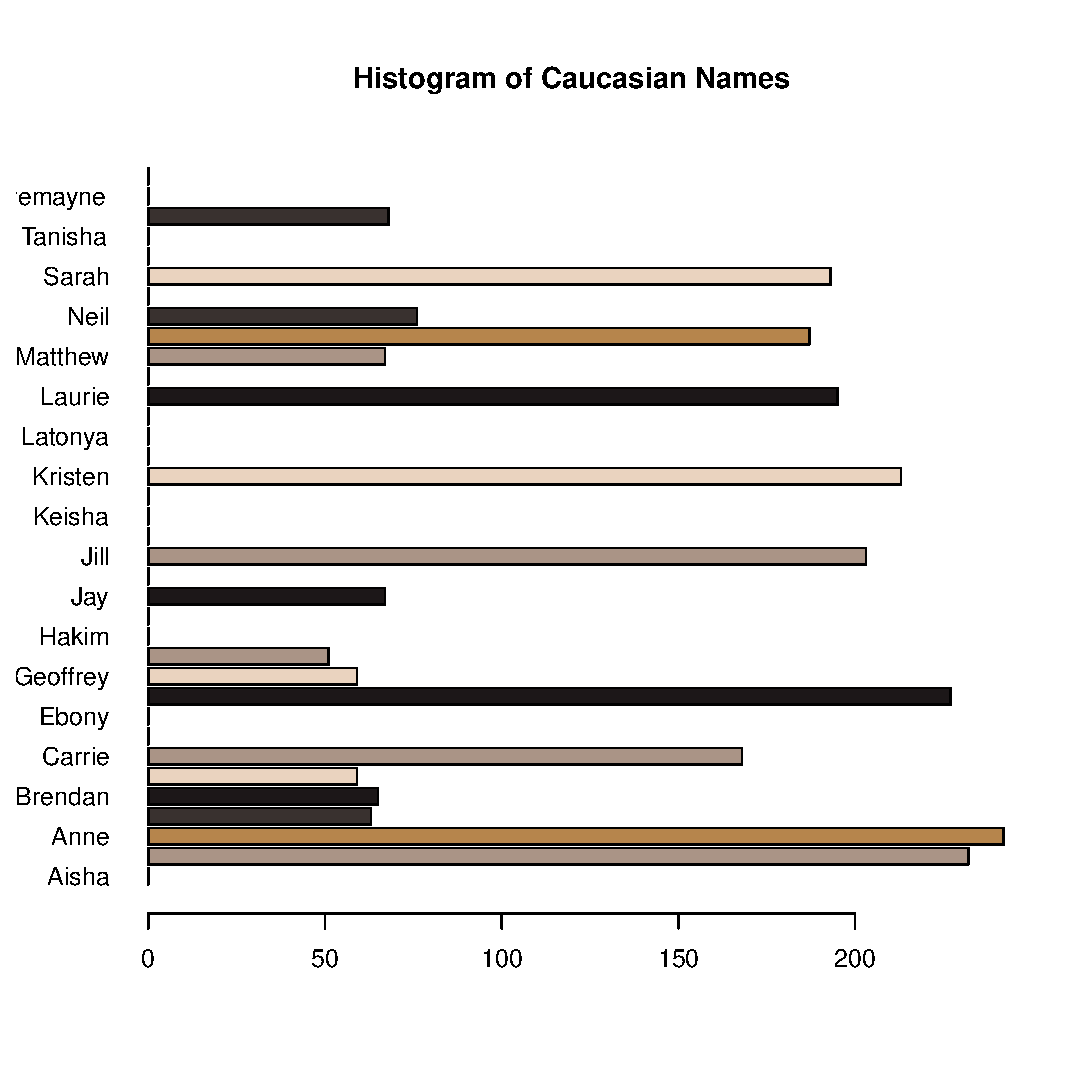
\includegraphics[width=\textwidth]{../Figures/Histogram - Names, Caucasian.eps}
\caption{Histogram of Caucasian Names}
\label{fig:whitenames}
\end{figure}


\begin{figure}
\centering
\includegraphics[width=\textwidth]{../Figures/Histogram - Names, African Americans.eps}
\caption{Histogram of African American Names}
\label{fig:blacknames}
\end{figure}


\begin{figure}
\centering
\includegraphics[width=\textwidth]{../Figures/Histogram - Names, Male.eps}
\caption{Histogram of Male Names}
\label{fig:malenames}
\end{figure}


\begin{figure}
\centering
\includegraphics[width=\textwidth]{../Figures/Histogram - Names, Female.eps}
\caption{Histogram of Female Names}
\label{fig:femalenames}
\end{figure}


Just to demonstrate how randomized the resumes were when the study was conducted, I have displayed this table below. This shows all of the resumes with the name Tanisha. Each resume has its own combination of criteria:


% latex table generated in R 3.6.1 by xtable 1.8-4 package
% Sat Dec 05 18:24:26 2020
\begin{table}[ht]
\centering
\begin{tabular}{rllllrlrrllllllllll}
  \hline
 & name & gender & ethnicity & quality & call & city & jobs & experience & holes & computer & college & minimum & equal & wanted & reqexp & reqeduc & reqcomp & industry \\ 
  \hline
127 & Tanisha & female & afam & high & 1.00 & chicago &   1 &   9 & no & yes & yes & some & no & supervisor & yes & no & no & trade \\ 
  171 & Tanisha & female & afam & low & 0.00 & chicago &   2 &   6 & no & yes & no & none & no & office support & no & no & yes & manufacturing \\ 
  172 & Tanisha & female & afam & low & 1.00 & chicago &   3 &  11 & yes & yes & no & none & yes & other & no & no & no & business/personal services \\ 
  198 & Tanisha & female & afam & high & 0.00 & boston &   4 &  14 & no & yes & yes & 3 & yes & manager & yes & yes & no & manufacturing \\ 
  199 & Tanisha & female & afam & high & 0.00 & boston &   6 &   8 & no & yes & yes & some & no & retail sales & yes & no & no & unknown \\ 
  224 & Tanisha & female & afam & high & 0.00 & chicago &   3 &  10 & no & yes & yes & some & no & secretary & yes & no & yes & business/personal services \\ 
  232 & Tanisha & female & afam & high & 0.00 & chicago &   4 &  21 & yes & yes & yes & 1 & no & office support & yes & no & no & business/personal services \\ 
  236 & Tanisha & female & afam & high & 0.00 & chicago &   3 &   5 & no & yes & no & 2 & no & secretary & yes & no & yes & health/education/social services \\ 
  254 & Tanisha & female & afam & low & 0.00 & chicago &   2 &  13 & yes & yes & yes & 3 & no & secretary & yes & yes & yes & unknown \\ 
  320 & Tanisha & female & afam & high & 0.00 & chicago &   3 &   6 & no & yes & no & 3 & no & secretary & yes & no & yes & business/personal services \\ 
  376 & Tanisha & female & afam & high & 0.00 & boston &   6 &   8 & no & yes & yes & none & no & retail sales & no & no & no & unknown \\ 
  394 & Tanisha & female & afam & low & 0.00 & boston &   2 &   1 & yes & yes & no & none & no & office support & no & no & yes & unknown \\ 
  420 & Tanisha & female & afam & low & 0.00 & boston &   3 &   7 & yes & yes & no & none & no & secretary & no & no & no & unknown \\ 
  436 & Tanisha & female & afam & high & 0.00 & boston &   6 &  16 & no & yes & no & none & no & secretary & no & no & yes & business/personal services \\ 
  472 & Tanisha & female & afam & low & 0.00 & chicago &   4 &  11 & no & yes & no & none & no & secretary & no & no & no & health/education/social services \\ 
  488 & Tanisha & female & afam & low & 0.00 & chicago &   4 &   4 & yes & yes & yes & 2 & no & secretary & yes & no & yes & business/personal services \\ 
  492 & Tanisha & female & afam & low & 0.00 & chicago &   2 &  10 & yes & yes & yes & none & no & supervisor & no & yes & yes & health/education/social services \\ 
  504 & Tanisha & female & afam & low & 0.00 & chicago &   2 &   6 & no & yes & yes & none & yes & office support & no & no & yes & manufacturing \\ 
  520 & Tanisha & female & afam & low & 0.00 & chicago &   4 &   6 & no & yes & no & none & no & secretary & no & no & no & finance/insurance/real estate \\ 
  570 & Tanisha & female & afam & low & 0.00 & boston &   3 &   8 & yes & no & no & 2 & no & other & yes & no & no & trade \\ 
  592 & Tanisha & female & afam & low & 0.00 & boston &   5 &  13 & no & yes & no & some & no & office support & yes & no & no & business/personal services \\ 
  600 & Tanisha & female & afam & low & 0.00 & boston &   5 &  13 & no & yes & no & none & no & office support & no & no & yes & health/education/social services \\ 
  604 & Tanisha & female & afam & high & 0.00 & boston &   4 &  18 & yes & yes & no & none & no & manager & no & no & no & business/personal services \\ 
  654 & Tanisha & female & afam & high & 0.00 & chicago &   4 &  11 & no & yes & yes & none & yes & secretary & no & no & yes & health/education/social services \\ 
  666 & Tanisha & female & afam & low & 0.00 & chicago &   2 &   3 & no & yes & yes & some & no & secretary & yes & no & yes & trade \\ 
  674 & Tanisha & female & afam & high & 0.00 & chicago &   4 &   5 & no & yes & yes & none & no & office support & no & no & yes & business/personal services \\ 
  682 & Tanisha & female & afam & low & 0.00 & chicago &   4 &   7 & no & yes & yes & none & yes & supervisor & no & no & no & trade \\ 
  694 & Tanisha & female & afam & high & 0.00 & chicago &   3 &   5 & yes & yes & yes & none & no & supervisor & no & no & yes & unknown \\ 
  723 & Tanisha & female & afam & low & 0.00 & boston &   3 &  10 & yes & no & no & none & no & other & no & no & no & trade \\ 
  724 & Tanisha & female & afam & high & 0.00 & boston &   4 &   2 & no & yes & yes & some & no & other & yes & no & no & unknown \\ 
  730 & Tanisha & female & afam & low & 0.00 & boston &   5 &  13 & yes & yes & no & some & no & secretary & yes & no & no & health/education/social services \\ 
  738 & Tanisha & female & afam & high & 0.00 & boston &   5 &  19 & no & no & no & some & no & office support & yes & no & no & business/personal services \\ 
  760 & Tanisha & female & afam & low & 0.00 & chicago &   4 &  11 & yes & yes & yes & none & no & other & no & no & no & business/personal services \\ 
  786 & Tanisha & female & afam & low & 0.00 & chicago &   5 &   6 & yes & yes & yes & none & no & secretary & no & no & no & business/personal services \\ 
  804 & Tanisha & female & afam & low & 0.00 & chicago &   2 &  15 & no & yes & yes & none & no & secretary & no & no & yes & unknown \\ 
  824 & Tanisha & female & afam & high & 0.00 & chicago &   3 &   5 & no & yes & no & none & no & secretary & no & no & yes & finance/insurance/real estate \\ 
  876 & Tanisha & female & afam & low & 0.00 & boston &   5 &   5 & yes & no & no & none & no & supervisor & no & no & yes & health/education/social services \\ 
  883 & Tanisha & female & afam & low & 0.00 & boston &   3 &   7 & yes & no & yes & none & yes & retail sales & no & no & no & manufacturing \\ 
  906 & Tanisha & female & afam & low & 0.00 & chicago &   4 &  15 & yes & yes & yes & none & no & office support & no & no & yes & business/personal services \\ 
  914 & Tanisha & female & afam & low & 0.00 & chicago &   2 &  11 & yes & yes & no & some & no & secretary & yes & no & no & finance/insurance/real estate \\ 
  968 & Tanisha & female & afam & low & 0.00 & chicago &   4 &   6 & yes & yes & yes & 3 & yes & secretary & yes & no & yes & business/personal services \\ 
  972 & Tanisha & female & afam & high & 0.00 & chicago &   5 &   8 & yes & yes & yes & some & no & secretary & yes & no & yes & business/personal services \\ 
  1034 & Tanisha & female & afam & high & 0.00 & boston &   6 &   8 & no & yes & yes & none & no & other & no & no & no & manufacturing \\ 
  1066 & Tanisha & female & afam & high & 0.00 & chicago &   4 &   8 & yes & yes & yes & 3 & no & secretary & yes & yes & no & finance/insurance/real estate \\ 
  1070 & Tanisha & female & afam & high & 0.00 & chicago &   3 &   6 & no & yes & yes & 1 & no & manager & yes & no & no & business/personal services \\ 
  1074 & Tanisha & female & afam & low & 0.00 & chicago &   4 &   6 & no & yes & no & none & no & office support & no & no & yes & business/personal services \\ 
  1102 & Tanisha & female & afam & high & 0.00 & chicago &   4 &   6 & yes & yes & yes & some & no & secretary & yes & no & yes & health/education/social services \\ 
  1118 & Tanisha & female & afam & low & 0.00 & chicago &   2 &  14 & no & yes & yes & 3 & yes & secretary & yes & no & yes & business/personal services \\ 
  1170 & Tanisha & female & afam & high & 0.00 & boston &   5 &  26 & yes & yes & no & none & no & secretary & no & no & no & health/education/social services \\ 
  1178 & Tanisha & female & afam & high & 0.00 & boston &   3 &   7 & yes & yes & yes & none & no & secretary & no & no & yes & business/personal services \\ 
  1186 & Tanisha & female & afam & high & 0.00 & boston &   6 &  16 & yes & yes & no & some & no & secretary & yes & no & no & business/personal services \\ 
  1206 & Tanisha & female & afam & low & 0.00 & chicago &   3 &   6 & yes & yes & yes & none & no & office support & no & no & no & business/personal services \\ 
  1218 & Tanisha & female & afam & high & 0.00 & chicago &   4 &   6 & yes & yes & no & none & no & secretary & no & no & yes & transport/communication \\ 
  1222 & Tanisha & female & afam & low & 0.00 & chicago &   4 &   6 & no & yes & no & none & no & secretary & no & no & no & business/personal services \\ 
  1226 & Tanisha & female & afam & low & 0.00 & chicago &   3 &   8 & yes & yes & no & some & yes & retail sales & yes & no & no & manufacturing \\ 
  1240 & Tanisha & female & afam & high & 0.00 & chicago &   4 &   7 & no & yes & yes & 5 & no & supervisor & yes & no & yes & trade \\ 
  1280 & Tanisha & female & afam & low & 0.00 & boston &   3 &   4 & yes & yes & no & none & no & secretary & no & no & no & business/personal services \\ 
  1320 & Tanisha & female & afam & high & 0.00 & chicago &   3 &   4 & no & yes & no & none & no & secretary & no & no & yes & health/education/social services \\ 
  1330 & Tanisha & female & afam & low & 0.00 & chicago &   4 &  11 & yes & no & yes & none & no & office support & no & no & yes & trade \\ 
  1334 & Tanisha & female & afam & low & 1.00 & chicago &   2 &   7 & yes & yes & yes & 3 & no & office support & yes & no & no & unknown \\ 
  1342 & Tanisha & female & afam & high & 0.00 & chicago &   4 &   6 & yes & yes & no & none & no & office support & no & no & yes & unknown \\ 
  1374 & Tanisha & female & afam & high & 0.00 & chicago &   4 &  11 & yes & yes & no & some & yes & supervisor & yes & no & yes & unknown \\ 
  1410 & Tanisha & female & afam & low & 1.00 & boston &   3 &   4 & yes & yes & no & none & no & secretary & no & no & yes & health/education/social services \\ 
  1414 & Tanisha & female & afam & high & 0.00 & boston &   1 &   5 & no & yes & yes & none & no & office support & no & no & yes & manufacturing \\ 
  1430 & Tanisha & female & afam & high & 0.00 & boston &   6 &   9 & yes & yes & yes & none & no & secretary & no & no & yes & health/education/social services \\ 
  1442 & Tanisha & female & afam & low & 0.00 & boston &   6 &   7 & yes & no & yes & none & no & secretary & no & no & no & business/personal services \\ 
  1446 & Tanisha & female & afam & high & 0.00 & boston &   3 &   8 & yes & yes & yes & none & no & secretary & no & no & yes & business/personal services \\ 
  1552 & Tanisha & female & afam & low & 0.00 & boston &   3 &   7 & yes & yes & no & none & no & secretary & no & no & no & health/education/social services \\ 
  1604 & Tanisha & female & afam & low & 0.00 & chicago &   3 &   5 & yes & yes & yes & none & no & office support & no & no & yes & manufacturing \\ 
  1680 & Tanisha & female & afam & high & 0.00 & boston &   6 &   8 & no & yes & yes & none & no & other & no & no & yes & business/personal services \\ 
  1686 & Tanisha & female & afam & low & 0.00 & boston &   6 &   7 & yes & no & yes & none & no & supervisor & no & no & no & business/personal services \\ 
  1710 & Tanisha & female & afam & high & 0.00 & boston &   5 &   9 & yes & yes & yes & none & no & office support & no & no & no & business/personal services \\ 
  1714 & Tanisha & female & afam & high & 0.00 & boston &   5 &  26 & yes & yes & no & some & no & secretary & yes & no & yes & trade \\ 
  1732 & Tanisha & female & afam & high & 0.00 & chicago &   2 &  12 & no & yes & no & none & no & secretary & no & no & yes & business/personal services \\ 
  1740 & Tanisha & female & afam & low & 0.00 & chicago &   2 &  11 & yes & yes & yes & 10 & yes & supervisor & yes & yes & yes & business/personal services \\ 
  1752 & Tanisha & female & afam & high & 0.00 & chicago &   4 &   9 & yes & yes & yes & none & no & supervisor & no & no & yes & business/personal services \\ 
  1788 & Tanisha & female & afam & low & 0.00 & chicago &   3 &   7 & yes & yes & no & 3 & yes & supervisor & yes & no & no & health/education/social services \\ 
  1799 & Tanisha & female & afam & high & 0.00 & chicago &   2 &   5 & yes & no & yes & none & no & retail sales & no & no & no & trade \\ 
  1814 & Tanisha & female & afam & high & 0.00 & chicago &   4 &   6 & no & yes & yes & none & yes & manager & no & yes & yes & business/personal services \\ 
  1836 & Tanisha & female & afam & low & 0.00 & chicago &   3 &   5 & yes & yes & no & 4 & yes & supervisor & yes & no & yes & unknown \\ 
  1842 & Tanisha & female & afam & high & 0.00 & chicago &   3 &  16 & no & yes & no & none & no & office support & no & no & yes & business/personal services \\ 
  1860 & Tanisha & female & afam & low & 0.00 & chicago &   4 &  11 & yes & yes & yes & none & no & secretary & no & no & yes & unknown \\ 
  1934 & Tanisha & female & afam & low & 0.00 & chicago &   1 &  13 & yes & yes & no & none & no & office support & no & no & no & business/personal services \\ 
  1944 & Tanisha & female & afam & high & 0.00 & chicago &   3 &  22 & no & yes & no & none & no & office support & no & no & no & manufacturing \\ 
  1948 & Tanisha & female & afam & low & 0.00 & chicago &   2 &  19 & yes & yes & yes & none & no & secretary & no & no & yes & health/education/social services \\ 
  2001 & Tanisha & female & afam & high & 0.00 & boston &   4 &   2 & no & yes & yes & some & no & other & yes & no & no & trade \\ 
  2008 & Tanisha & female & afam & low & 0.00 & boston &   3 &   7 & yes & yes & no & none & no & secretary & no & no & no & health/education/social services \\ 
  2020 & Tanisha & female & afam & high & 0.00 & boston &   2 &   6 & yes & yes & yes & none & no & other & no & no & no & unknown \\ 
  2032 & Tanisha & female & afam & high & 0.00 & chicago &   3 &  21 & yes & yes & no & none & no & secretary & no & no & no & trade \\ 
  2092 & Tanisha & female & afam & low & 0.00 & boston &   4 &  11 & yes & yes & yes & some & no & secretary & yes & no & yes & health/education/social services \\ 
  2096 & Tanisha & female & afam & low & 0.00 & boston &   2 &   2 & yes & no & no & none & yes & secretary & no & no & no & trade \\ 
  2116 & Tanisha & female & afam & low & 0.00 & chicago &   3 &   8 & yes & yes & no & 2 & no & secretary & yes & no & yes & unknown \\ 
  2124 & Tanisha & female & afam & low & 0.00 & chicago &   4 &   6 & yes & yes & yes & none & no & office support & no & no & no & health/education/social services \\ 
  2187 & Tanisha & female & afam & low & 0.00 & boston &   4 &   6 & no & yes & yes & none & yes & other & no & no & no & unknown \\ 
  2188 & Tanisha & female & afam & high & 0.00 & boston &   4 &   2 & no & yes & yes & none & no & other & no & no & no & manufacturing \\ 
  2196 & Tanisha & female & afam & high & 0.00 & boston &   1 &   5 & no & yes & yes & none & yes & secretary & no & yes & yes & health/education/social services \\ 
  2256 & Tanisha & female & afam & low & 1.00 & chicago &   4 &   2 & yes & yes & yes & none & no & secretary & no & no & yes & health/education/social services \\ 
  2264 & Tanisha & female & afam & low & 0.00 & chicago &   2 &  14 & no & yes & yes & none & no & secretary & no & yes & yes & unknown \\ 
  2299 & Tanisha & female & afam & high & 0.00 & boston &   4 &   2 & no & yes & yes & none & no & other & no & no & no & trade \\ 
  2316 & Tanisha & female & afam & high & 0.00 & boston &   5 &  19 & no & no & no & none & no & supervisor & no & no & no & health/education/social services \\ 
  2376 & Tanisha & female & afam & high & 1.00 & boston &   4 &  13 & yes & yes & yes & 5 & yes & secretary & yes & yes & no & health/education/social services \\ 
  2426 & Tanisha & female & afam & high & 0.00 & chicago &   4 &   7 & no & yes & yes & 5 & no & secretary & yes & no & yes & business/personal services \\ 
  2430 & Tanisha & female & afam & low & 0.00 & chicago &   2 &   4 & no & yes & yes & some & no & secretary & yes & no & yes & unknown \\ 
  2470 & Tanisha & female & afam & high & 1.00 & boston &   5 &   9 & yes & yes & yes & none & no & secretary & no & no & yes & business/personal services \\ 
  2538 & Tanisha & female & afam & low & 0.00 & boston &   3 &   4 & yes & yes & no & none & no & supervisor & no & no & yes & business/personal services \\ 
  2550 & Tanisha & female & afam & high & 1.00 & boston &   5 &  14 & yes & yes & yes & none & no & secretary & no & no & no & health/education/social services \\ 
  2554 & Tanisha & female & afam & high & 0.00 & boston &   4 &   4 & no & yes & yes & none & no & other & no & no & no & unknown \\ 
  2593 & Tanisha & female & afam & low & 0.00 & boston &   4 &   6 & no & yes & yes & 2 & no & other & yes & yes & no & manufacturing \\ 
  2594 & Tanisha & female & afam & low & 0.00 & boston &   3 &   7 & yes & no & yes & none & no & other & no & no & no & manufacturing \\ 
  2595 & Tanisha & female & afam & high & 0.00 & boston &   7 &   5 & no & yes & yes & 2 & no & retail sales & yes & no & no & business/personal services \\ 
  2604 & Tanisha & female & afam & low & 0.00 & boston &   5 &  13 & yes & yes & no & none & no & office support & no & no & yes & finance/insurance/real estate \\ 
  2620 & Tanisha & female & afam & high & 0.00 & boston &   5 &  19 & no & no & no & none & no & supervisor & no & no & no & health/education/social services \\ 
  2628 & Tanisha & female & afam & high & 1.00 & boston &   6 &  16 & no & yes & no & none & no & office support & no & no & yes & health/education/social services \\ 
  2674 & Tanisha & female & afam & high & 0.00 & boston &   1 &   5 & no & yes & yes & none & no & office support & no & no & yes & business/personal services \\ 
  2704 & Tanisha & female & afam & low & 0.00 & chicago &   4 &   6 & no & yes & yes & 3 & yes & secretary & yes & yes & yes & health/education/social services \\ 
  2736 & Tanisha & female & afam & low & 0.00 & boston &   2 &   2 & yes & no & no & none & no & secretary & no & no & no & business/personal services \\ 
  2740 & Tanisha & female & afam & low & 0.00 & boston &   5 &   4 & yes & yes & no & none & no & office support & no & no & no & unknown \\ 
  2744 & Tanisha & female & afam & high & 0.00 & boston &   5 &   9 & yes & yes & yes & none & no & office support & no & no & yes & business/personal services \\ 
  2776 & Tanisha & female & afam & low & 0.00 & chicago &   2 &   4 & yes & yes & yes & 3 & no & manager & yes & no & yes & unknown \\ 
  2780 & Tanisha & female & afam & high & 0.00 & chicago &   3 &  11 & no & yes & yes & none & yes & secretary & no & no & yes & trade \\ 
  2782 & Tanisha & female & afam & low & 0.00 & chicago &   3 &   4 & no & yes & yes & none & no & retail sales & no & no & no & business/personal services \\ 
  2808 & Tanisha & female & afam & high & 0.00 & chicago &   2 &   5 & no & no & yes & none & no & retail sales & no & no & no & trade \\ 
  2836 & Tanisha & female & afam & low & 0.00 & chicago &   4 &   6 & yes & yes & yes & 2 & no & secretary & yes & no & yes & health/education/social services \\ 
  2872 & Tanisha & female & afam & high & 0.00 & chicago &   4 &  11 & no & yes & yes & 10 & no & supervisor & yes & no & yes & business/personal services \\ 
  2880 & Tanisha & female & afam & high & 0.00 & chicago &   3 &   7 & no & yes & no & 6 & yes & secretary & yes & no & yes & manufacturing \\ 
  2892 & Tanisha & female & afam & high & 0.00 & chicago &   3 &   7 & no & yes & yes & some & yes & manager & yes & yes & yes & trade \\ 
  2898 & Tanisha & female & afam & high & 0.00 & chicago &   3 &   3 & no & yes & no & none & yes & secretary & no & no & yes & manufacturing \\ 
  2902 & Tanisha & female & afam & high & 0.00 & chicago &   4 &   8 & no & yes & yes & 3 & yes & supervisor & yes & no & yes & health/education/social services \\ 
  2907 & Tanisha & female & afam & high & 0.00 & chicago &   3 &  16 & no & yes & no & none & no & secretary & no & no & yes & health/education/social services \\ 
  2916 & Tanisha & female & afam & low & 0.00 & chicago &   3 &   4 & no & no & yes & none & no & manager & no & no & no & trade \\ 
  2946 & Tanisha & female & afam & high & 0.00 & chicago &   3 &   6 & no & yes & yes & none & no & secretary & no & no & yes & business/personal services \\ 
  3017 & Tanisha & female & afam & high & 0.00 & boston &   6 &   8 & no & yes & yes & none & no & retail sales & no & no & no & unknown \\ 
  3022 & Tanisha & female & afam & low & 0.00 & boston &   3 &   7 & yes & yes & no & none & no & office support & no & no & no & health/education/social services \\ 
  3030 & Tanisha & female & afam & low & 0.00 & boston &   3 &   7 & yes & yes & no & some & no & secretary & yes & no & no & health/education/social services \\ 
  3034 & Tanisha & female & afam & low & 0.00 & boston &   5 &   4 & yes & yes & no & none & no & secretary & no & no & no & unknown \\ 
  3050 & Tanisha & female & afam & low & 0.00 & chicago &   2 &   6 & no & yes & yes & none & no & office support & no & no & yes & unknown \\ 
  3074 & Tanisha & female & afam & low & 0.00 & boston &   5 &   5 & yes & no & no & none & no & secretary & no & no & yes & business/personal services \\ 
  3094 & Tanisha & female & afam & low & 0.00 & boston &   4 &  11 & yes & yes & yes & some & no & secretary & yes & no & yes & business/personal services \\ 
  3119 & Tanisha & female & afam & low & 0.00 & boston &   4 &   8 & no & no & yes & none & no & other & no & no & no & transport/communication \\ 
  3177 & Tanisha & female & afam & low & 0.00 & boston &   3 &   7 & yes & no & yes & some & no & retail sales & yes & no & no & trade \\ 
  3234 & Tanisha & female & afam & high & 0.00 & boston &   2 &  10 & yes & yes & yes & 1 & yes & retail sales & yes & no & no & business/personal services \\ 
  3274 & Tanisha & female & afam & low & 0.00 & chicago &   2 &   4 & yes & yes & no & none & no & secretary & no & no & yes & finance/insurance/real estate \\ 
  3292 & Tanisha & female & afam & high & 0.00 & chicago &   4 &   7 & yes & yes & no & none & no & secretary & no & yes & no & business/personal services \\ 
  3298 & Tanisha & female & afam & high & 0.00 & chicago &   4 &   8 & no & yes & yes & none & no & other & no & no & no & finance/insurance/real estate \\ 
  3320 & Tanisha & female & afam & high & 0.00 & chicago &   3 &   8 & no & yes & yes & none & no & secretary & no & no & yes & health/education/social services \\ 
  3334 & Tanisha & female & afam & high & 0.00 & chicago &   3 &   6 & no & yes & yes & 3 & yes & secretary & yes & no & yes & trade \\ 
  3370 & Tanisha & female & afam & high & 0.00 & chicago &   4 &   5 & yes & yes & yes & 3 & yes & secretary & yes & no & yes & trade \\ 
  3392 & Tanisha & female & afam & low & 0.00 & chicago &   2 &   5 & no & no & no & some & no & secretary & yes & yes & yes & health/education/social services \\ 
  3413 & Tanisha & female & afam & low & 0.00 & chicago &   2 &   4 & yes & yes & yes & 2 & yes & secretary & yes & no & yes & trade \\ 
  3464 & Tanisha & female & afam & low & 0.00 & boston &   2 &  10 & yes & yes & yes & 1 & no & manager & yes & no & no & transport/communication \\ 
  3481 & Tanisha & female & afam & low & 0.00 & boston &   3 &   7 & yes & no & yes & 10 & no & retail sales & yes & no & no & trade \\ 
  3566 & Tanisha & female & afam & low & 0.00 & boston &   4 &   6 & no & yes & yes & none & no & other & no & no & no & trade \\ 
  3602 & Tanisha & female & afam & high & 0.00 & boston &   3 &   7 & yes & yes & yes & 2 & no & secretary & yes & no & yes & business/personal services \\ 
  3610 & Tanisha & female & afam & low & 0.00 & boston &   3 &   7 & yes & no & yes & none & yes & retail sales & no & no & no & trade \\ 
  3621 & Tanisha & female & afam & low & 0.00 & boston &   3 &   7 & yes & no & yes & none & no & retail sales & no & no & no & trade \\ 
  3622 & Tanisha & female & afam & high & 0.00 & boston &   4 &   2 & no & yes & yes & some & yes & retail sales & yes & no & no & trade \\ 
  3644 & Tanisha & female & afam & high & 0.00 & chicago &   3 &   5 & no & yes & yes & none & no & office support & no & no & yes & finance/insurance/real estate \\ 
  3674 & Tanisha & female & afam & low & 0.00 & chicago &   4 &   6 & no & yes & yes & none & no & supervisor & no & yes & yes & unknown \\ 
  3678 & Tanisha & female & afam & low & 0.00 & chicago &   3 &   4 & yes & yes & yes & none & no & secretary & no & yes & yes & business/personal services \\ 
  3720 & Tanisha & female & afam & high & 0.00 & chicago &   4 &  11 & no & yes & yes & none & yes & office support & no & no & yes & manufacturing \\ 
  3734 & Tanisha & female & afam & low & 0.00 & chicago &   4 &   6 & yes & yes & yes & some & no & secretary & yes & no & yes & business/personal services \\ 
  3764 & Tanisha & female & afam & high & 0.00 & chicago &   4 &   5 & no & yes & yes & none & yes & secretary & no & no & yes & trade \\ 
  3770 & Tanisha & female & afam & high & 0.00 & chicago &   3 &   3 & no & yes & no & some & no & supervisor & yes & no & yes & finance/insurance/real estate \\ 
  3786 & Tanisha & female & afam & low & 0.00 & chicago &   2 &   4 & no & no & yes & none & no & retail sales & no & no & no & trade \\ 
  3790 & Tanisha & female & afam & low & 0.00 & chicago &   4 &   6 & no & yes & no & none & yes & office support & no & no & no & manufacturing \\ 
  3831 & Tanisha & female & afam & low & 0.00 & boston &   4 &   6 & no & yes & yes & none & yes & retail sales & no & yes & no & business/personal services \\ 
  3858 & Tanisha & female & afam & high & 0.00 & boston &   6 &   8 & no & yes & yes & none & no & retail sales & no & no & no & unknown \\ 
  3884 & Tanisha & female & afam & low & 0.00 & boston &   4 &   6 & no & yes & yes & some & yes & other & yes & yes & no & finance/insurance/real estate \\ 
  3948 & Tanisha & female & afam & high & 0.00 & chicago &   3 &   5 & no & yes & no & none & yes & secretary & no & no & yes & business/personal services \\ 
  3960 & Tanisha & female & afam & high & 0.00 & chicago &   3 &   7 & yes & yes & yes & none & no & secretary & no & no & yes & trade \\ 
  3978 & Tanisha & female & afam & high & 0.00 & chicago &   3 &   3 & no & yes & yes & none & yes & retail sales & no & no & no & transport/communication \\ 
  3994 & Tanisha & female & afam & low & 0.00 & chicago &   3 &   3 & yes & yes & yes & some & no & manager & yes & no & no & business/personal services \\ 
  4014 & Tanisha & female & afam & high & 0.00 & chicago &   4 &   7 & no & yes & yes & none & yes & secretary & no & yes & yes & health/education/social services \\ 
  4018 & Tanisha & female & afam & low & 0.00 & chicago &   2 &   6 & no & yes & yes & some & yes & secretary & yes & yes & yes & health/education/social services \\ 
  4024 & Tanisha & female & afam & high & 0.00 & chicago &   3 &  15 & no & yes & no & none & yes & secretary & no & no & yes & finance/insurance/real estate \\ 
  4040 & Tanisha & female & afam & low & 0.00 & chicago &   3 &   8 & yes & yes & no & some & no & secretary & yes & no & no & finance/insurance/real estate \\ 
  4055 & Tanisha & female & afam & high & 0.00 & chicago &   3 &   2 & no & yes & yes & 3 & no & retail sales & yes & no & no & trade \\ 
  4078 & Tanisha & female & afam & high & 0.00 & chicago &   3 &   8 & yes & yes & yes & 3 & no & supervisor & yes & no & no & health/education/social services \\ 
  4134 & Tanisha & female & afam & high & 0.00 & boston &   5 &  18 & yes & no & no & none & no & office support & no & no & yes & business/personal services \\ 
  4169 & Tanisha & female & afam & high & 1.00 & boston &   4 &   2 & no & yes & yes & some & no & retail sales & yes & no & yes & trade \\ 
  4188 & Tanisha & female & afam & high & 0.00 & chicago &   3 &   4 & no & yes & no & 3 & no & secretary & yes & no & no & health/education/social services \\ 
  4201 & Tanisha & female & afam & low & 0.00 & chicago &   3 &   6 & yes & yes & yes & 3 & yes & secretary & yes & no & yes & unknown \\ 
  4206 & Tanisha & female & afam & high & 0.00 & chicago &   3 &  13 & no & yes & no & none & yes & secretary & no & no & yes & business/personal services \\ 
  4258 & Tanisha & female & afam & high & 0.00 & chicago &   3 &   5 & no & yes & no & none & no & manager & no & no & no & trade \\ 
  4282 & Tanisha & female & afam & low & 0.00 & chicago &   4 &   5 & no & yes & no & none & yes & secretary & no & no & yes & health/education/social services \\ 
  4306 & Tanisha & female & afam & high & 0.00 & chicago &   3 &   5 & no & yes & no & none & no & secretary & no & no & yes & finance/insurance/real estate \\ 
  4326 & Tanisha & female & afam & high & 0.00 & chicago &   4 &   9 & yes & yes & yes & 0.5 & yes & office support & yes & yes & yes & health/education/social services \\ 
  4336 & Tanisha & female & afam & low & 1.00 & chicago &   5 &   8 & yes & yes & yes & none & no & office support & no & no & no & health/education/social services \\ 
  4372 & Tanisha & female & afam & low & 0.00 & boston &   4 &   6 & no & yes & yes & none & yes & retail sales & no & no & no & manufacturing \\ 
  4376 & Tanisha & female & afam & high & 0.00 & boston &   5 &  26 & yes & yes & no & none & no & secretary & no & no & yes & unknown \\ 
  4404 & Tanisha & female & afam & high & 1.00 & boston &   6 &  18 & no & yes & yes & 2 & yes & manager & yes & no & no & business/personal services \\ 
  4422 & Tanisha & female & afam & high & 0.00 & chicago &   3 &   7 & no & yes & yes & 5 & yes & secretary & yes & yes & yes & health/education/social services \\ 
  4468 & Tanisha & female & afam & high & 0.00 & chicago &   5 &   7 & yes & yes & yes & none & no & secretary & no & no & no & unknown \\ 
  4480 & Tanisha & female & afam & low & 0.00 & boston &   2 &   2 & yes & no & no & none & no & supervisor & no & no & yes & finance/insurance/real estate \\ 
  4492 & Tanisha & female & afam & high & 0.00 & chicago &   4 &   7 & no & yes & yes & 1 & yes & other & yes & no & yes & unknown \\ 
  4506 & Tanisha & female & afam & high & 0.00 & chicago &   5 &   8 & yes & yes & yes & some & yes & office support & yes & no & yes & business/personal services \\ 
  4510 & Tanisha & female & afam & low & 0.00 & chicago &   4 &   5 & no & yes & no & none & yes & secretary & no & no & yes & health/education/social services \\ 
  4520 & Tanisha & female & afam & low & 0.00 & chicago &   4 &   6 & no & yes & no & none & no & secretary & no & no & yes & manufacturing \\ 
  4530 & Tanisha & female & afam & low & 0.00 & chicago &   4 &   6 & yes & yes & yes & 2 & yes & secretary & yes & no & yes & unknown \\ 
  4558 & Tanisha & female & afam & low & 0.00 & chicago &   4 &   4 & yes & yes & no & none & no & retail sales & no & no & no & finance/insurance/real estate \\ 
  4591 & Tanisha & female & afam & low & 0.00 & boston &   4 &   6 & no & yes & yes & some & no & other & yes & no & no & finance/insurance/real estate \\ 
  4622 & Tanisha & female & afam & low & 0.00 & boston &   5 &   5 & yes & no & no & none & no & office support & no & no & no & health/education/social services \\ 
  4689 & Tanisha & female & afam & low & 0.00 & chicago &   4 &   5 & yes & yes & yes & none & no & supervisor & no & no & no & transport/communication \\ 
  4754 & Tanisha & female & afam & low & 0.00 & chicago &   3 &   5 & no & yes & no & some & no & secretary & yes & no & yes & trade \\ 
  4772 & Tanisha & female & afam & low & 0.00 & chicago &   3 &   3 & yes & yes & no & 10 & no & supervisor & yes & no & yes & business/personal services \\ 
  4819 & Tanisha & female & afam & high & 0.00 & boston &   6 &   8 & no & yes & yes & 3 & yes & other & yes & yes & no & manufacturing \\ 
  4854 & Tanisha & female & afam & high & 0.00 & boston &   7 &  18 & yes & yes & no & none & no & supervisor & no & no & no & business/personal services \\ 
   \hline
\end{tabular}
\caption{Resumes under one name are randomized} 
\label{tab:SampleData}
\end{table}



\section{Logistic Regression Model}


After reviewing the data and some of the variables' statistics, I created a logistic regression model to fit to the dataset. Below are the results of the model:


% latex table generated in R 3.6.1 by xtable 1.8-4 package
% Sat Dec 05 18:24:26 2020
\begin{table}[ht]
\centering
\begin{tabular}{rrrrr}
  \hline
 & Estimate & Std. Error & z value & Pr($>$$|$z$|$) \\ 
  \hline
(Intercept) & 21.90 & 18789.26 & 0.00 & 1.00 \\ 
  gendermale & 18.44 & 775.34 & 0.02 & 0.98 \\ 
  ethnicitycauc & 18.95 & 559.15 & 0.03 & 0.97 \\ 
  qualitylow & -0.26 & 0.17 & -1.52 & 0.13 \\ 
  citychicago & -0.52 & 0.22 & -2.40 & 0.02 \\ 
  jobs & -0.13 & 0.08 & -1.58 & 0.11 \\ 
  experience & 0.05 & 0.02 & 2.30 & 0.02 \\ 
  holesyes & -0.27 & 0.17 & -1.57 & 0.12 \\ 
  computeryes & -0.35 & 0.28 & -1.23 & 0.22 \\ 
  collegeyes & 0.13 & 0.18 & 0.72 & 0.47 \\ 
  minimum0.5 & 18.25 & 16406.28 & 0.00 & 1.00 \\ 
  minimum1 & -0.91 & 13871.32 & -0.00 & 1.00 \\ 
  minimum10 & -1.45 & 13871.32 & -0.00 & 1.00 \\ 
  minimum2 & 0.28 & 13871.32 & 0.00 & 1.00 \\ 
  minimum3 & -0.19 & 13871.32 & -0.00 & 1.00 \\ 
  minimum4 & 18.26 & 16646.17 & 0.00 & 1.00 \\ 
  minimum5 & -0.51 & 13871.32 & -0.00 & 1.00 \\ 
  minimum6 & -1.47 & 13871.32 & -0.00 & 1.00 \\ 
  minimum7 & -0.96 & 13871.32 & -0.00 & 1.00 \\ 
  minimum8 & 18.01 & 16172.90 & 0.00 & 1.00 \\ 
  minimumnone & -19.00 & 18789.26 & -0.00 & 1.00 \\ 
  minimumsome & -0.34 & 13871.32 & -0.00 & 1.00 \\ 
  equalyes & -0.28 & 0.19 & -1.52 & 0.13 \\ 
  wantedoffice support & 0.70 & 0.35 & 2.03 & 0.04 \\ 
  wantedother & 0.06 & 0.34 & 0.17 & 0.86 \\ 
  wantedretail sales & 0.12 & 0.33 & 0.37 & 0.71 \\ 
  wantedsecretary & 0.32 & 0.28 & 1.17 & 0.24 \\ 
  wantedsupervisor & 0.57 & 0.37 & 1.55 & 0.12 \\ 
  reqexpyes & -18.75 & 12673.71 & -0.00 & 1.00 \\ 
  reqeducyes & -0.20 & 0.25 & -0.78 & 0.43 \\ 
  reqcompyes & 0.23 & 0.20 & 1.16 & 0.25 \\ 
  industryfinance/insurance/real estate & 0.09 & 0.30 & 0.29 & 0.77 \\ 
  industryhealth/education/social services & 0.08 & 0.25 & 0.31 & 0.76 \\ 
  industrymanufacturing & -0.05 & 0.32 & -0.15 & 0.88 \\ 
  industrytrade & 0.10 & 0.26 & 0.37 & 0.71 \\ 
  industrytransport/communication & -0.49 & 0.45 & -1.08 & 0.28 \\ 
  industryunknown & -0.02 & 0.25 & -0.08 & 0.94 \\ 
   \hline
\end{tabular}
\caption{Logistic Regression Model Summary} 
\label{tab:Model_Summary}
\end{table}




%% Logistic Regression Model Analysis:



Based on the p values of the model, ethnicity or gender had no significance in determining 
(the likelihood of receiving a call back from the employers. The most significant independent 
(variables were the city (primarily if the city was Chicago), the years of experience listed on 
(resume, and if the employer wanted to fill an office support position.
( 



\section{Data Dictionary}


For reference, here are explanations and definitions for some of the less obvious independent variables:



%% Explanations and Definitions of Variables:



Name, gender, ethnicity, city, and industry are self-explanatory so I will not list those definitions.
(quality = quality of resume 
(jobs = number of jobs listed on resume), the years of experience listed on 
(experience = number of years of work experience
(holes = does resume have some employment holes?
(computer = does resume mention some computer skills?
(college = does applicant have a college degree or more?
(minimum = minimum experience requirement of employer
(equal = is the employer EOE (Equal Opportunity Employment)?
(wanted = type of position desired by employer
(reqexp = does ad mention some experience requirement?
(reqeduc = does ad mention some educational requirement?
(reqcomp = does ad mention some computer skills requirement?
( 





%%%%%%%%%%%%%%%%%%%%%%%%%%%%%%%%%%%%%%%%
\end{document}
%%%%%%%%%%%%%%%%%%%%%%%%%%%%%%%%%%%%%%%%